\documentclass[tikz]{standalone}
\usepackage{pgfplots}
\pgfplotsset{compat=1.15}
\usepackage{mathrsfs}
\usetikzlibrary{arrows,calc}
\usepackage{tkz-euclide}

\pagestyle{empty}

\definecolor{AngleClr}{rgb}{0,0.39215686274509803,0}
\definecolor{ShapeClr}{rgb}{0.6,0.2,0}

\begin{document}

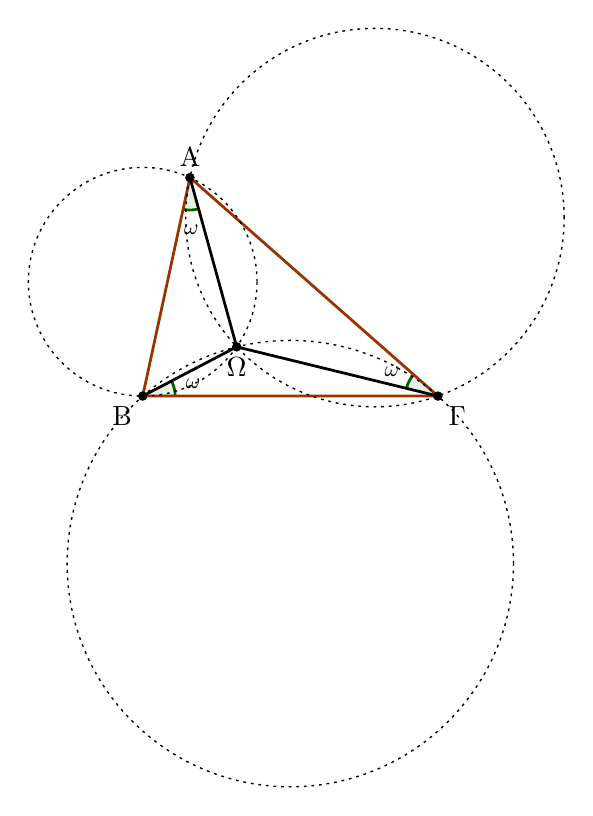
\begin{tikzpicture}[scale=.75]
\tkzSetUpLine[line width=1pt,color=black]
\tkzSetUpPoint[fill=black]

\tkzDefPoints{0/0/B,0.8/3.7/A,5/0/C}

\tkzDefMidPoint(B,C) \tkzGetPoint{MA}
\tkzDefMidPoint(A,C) \tkzGetPoint{MB}
\tkzDefMidPoint(B,A) \tkzGetPoint{MC}


\tkzDefLine[perpendicular=through B](B,C) \tkzGetPoint{BB}
\tkzDefLine[perpendicular=through MC](A,B) \tkzGetPoint{MMC}
\tkzInterLL(B,BB)(MC,MMC) \tkzGetPoint{OB}

\tkzDefLine[perpendicular=through C](C,A) \tkzGetPoint{CC}
\tkzDefLine[perpendicular=through MA](B,C) \tkzGetPoint{MMA}
\tkzInterLL(C,CC)(MA,MMA) \tkzGetPoint{OC}

\tkzDefLine[perpendicular=through A](A,B) \tkzGetPoint{AA}
\tkzDefLine[perpendicular=through MB](C,A) \tkzGetPoint{MMB}
\tkzInterLL(A,AA)(MB,MMB) \tkzGetPoint{OA}

\tkzInterCC(OA,A)(OB,B) \tkzGetPoints{Br1}{X}


\tkzFillPolygon[fill=white](A,B,C)

\tkzFillAngle[fill=AngleClr,size=.55,fill opacity=0.1](B,A,Br1)
\tkzMarkAngle[line width=1pt,size=.55,color=AngleClr](B,A,Br1)
\tkzLabelAngles[scale=0.8,pos=1.1](B,A,Br1){$\omega$}

\tkzFillAngle[fill=AngleClr,size=.55,fill opacity=0.1](C,B,Br1)
\tkzMarkAngle[line width=1pt,size=.55,color=AngleClr](C,B,Br1)
\tkzLabelAngles[scale=0.8,pos=1.1](C,B,Br1){$\omega$}

\tkzFillAngle[fill=AngleClr,size=.55,fill opacity=0.1](A,C,Br1)
\tkzMarkAngle[line width=1pt,size=.55,color=AngleClr](A,C,Br1)
\tkzLabelAngles[scale=0.8,pos=1.1](A,C,Br1){$\omega$}

\tkzDrawPolygon[color=ShapeClr](A,B,C)

\tkzDrawCircle[color=black,line width=0.5pt,dashed,dash pattern=on 1pt off 1.75pt](OA,A)
\tkzDrawCircle[color=black,line width=0.5pt,dashed,dash pattern=on 1pt off 1.75pt](OB,B)
\tkzDrawCircle[color=black,line width=0.5pt,dashed,dash pattern=on 1pt off 1.75pt](OC,C)

\tkzDrawSegments(Br1,A Br1,B Br1,C)

\tkzDrawPoints[size=3](A,B,C,Br1)

\tkzLabelPoint[above](A){$\mathrm{A}$}
\tkzLabelPoint[below left](B){$\mathrm{B}$}
\tkzLabelPoint[below right](C){$\mathrm{\Gamma}$}

\tkzLabelPoint[below](Br1){$\mathrm{\Omega}$}

\end{tikzpicture}
\end{document}
